\documentclass{article}

\usepackage[utf8]{inputenc}
\usepackage[round]{natbib}
\usepackage{fullpage}
\usepackage{longtable}
\usepackage{pdflscape}
\usepackage[margin=1in]{geometry}
\usepackage{graphicx}
\usepackage{authblk}
\usepackage{array}
\usepackage{ragged2e}
\usepackage{booktabs}
\usepackage{parskip}

\newcolumntype{P}[1]{>{\RaggedRight\hspace{0pt}}p{#1}}
\newcolumntype{X}[1]{>{\centering\arraybackslash\hspace{0pt}}p{#1}}




%\setlength{\parskip}{.8em}

\title{Supplementary material to "Why do we have so many different hydrological models? A review based on the case of Switzerland"}
\author[1]{Pascal Horton}
\author[1]{Bettina Schaefli}
\author[1]{Martina Kauzlaric}
\affil[1]{Institute of Geography \& Oeschger Centre for Climate Change Research, University of Bern, Bern, Switzerland}
\date{}

\begin{document}
	
\maketitle

\begin{abstract}
	This supplementary material contains two parts: first an extended version of the history of hydrological modelling in Switzerland, and second a table listing all modelling papers that were used for the analysis of Section 3 of the main paper (related to applications of hydrological models in Switzerland).
\end{abstract}



\section{History of hydrological modelling in Switzerland}


\subsection{Preliminary remark}

There was a journal entitled "Schweizerische Zeitschrift für Hydrologie" (Swiss journal for hydrology), published by Springer. The first issue of this journal was published in 1920 and called then "Zeitschrift für Hydrologie" (journal of hydrology). The journal changed its name in 1949 to Swiss journal of hydrology. It became "Aquatic sciences" in 1989 \citep{bossard1989} and is since then indexed on WebOfScience. The journal never had a particular focus on what we call hydrology today but was rooted in limnology and the hydrology of lakes \citep{tockner2009}. The name was chosen in 1920 by the then called Swiss Hydrobiological Commission (Swiss Society for Hydrology and Limnology today) \citep{perret2001} despite of being strongly rooted in limnology at that time. Accordingly, the Swiss journal for hydrology does not appear here in this brief overview.


\subsection{History of hydrological modelling in Switzerland}

On WebOfScience, the very first hydrological modelling paper that refers to Switzerland (index search: hydrolog* and model* and Switzerland or Swiss) was published by \citet{baumgartner1986} and was a proof of method for the use of remote sensing data for snow runoff modelling with the Snowmelt Runoff Model \citep[SRM,][]{martinec1975}. Journal of Hydrology has nevertheless published an earlier Swiss modelling paper, the work of \citet{hager1984}, who used a no-name conceptual model to predict the effect of heavy rainfall on an 8~km\textsuperscript{2} catchment in the Swiss lowlands.

Digging into professional journals and doctoral theses and conducting personal enquiries revealed the early hydrological modelling work of \citet{naef1974} for engineering applications. The work of Naef in particular also includes a very early hydrological model intercomparison study \citep{naef1977} where the behaviour of several conceptual models have been tested for three small well-instrumented catchments to understand if complex models yield better results than very simple ones.

The above work on input-output models (the focus of the main paper) in the 1970-1980ies was preceded by regression-based methods for real-time forecasting, specifically for inflow to hydropower plants \citep{jensenlang1973} and streamflow in the River Rhine \citep[e.g. to predict downstream summer droughts,][]{lugiez1969}.

Most of the early modelling work on streamflow with models representing hydrological processes (rather than purely statistical models) aimed at the development of operational forecast procedures and had a strong focus on snowmelt runoff and related streamflow, including in the lowland \citep{braun1986}. Snowmelt modelling probably started with the work of \citet{hoeck1952}, and modelling of snow runoff kept a strong influence on hydrological model development in the following decades.

The work of \citet{braun1986} combined the well-known temperature-index snow model \citep[underlying also the SRM model;][]{martinec1975} to the simplest possible streamflow transformation model, which assumes that half of the snowmelt during a given time step reaches the stream directly and the other half reaches it following a linear recession. This simplified approach (compared to more recent runoff transformation routines that use a recession coefficient as in SRM), dates back to the work of \citet{martinec1970} on snowmelt runoff modelling, which is thus probably the earliest runoff modelling study in Switzerland. 

Early modelling work also included glacier-melt runoff simulation \citep[][who used a model called HBV3-ETH, not in use anymore]{braun90}. \citet{braun1992} completed first attempts of parameter regionalization, i.e. the transfer of model parameters from one catchment to another, based on catchment characteristics. The work of \citet{hottelet1993} is an early example of model adaptation to a specific catchment; they added three parameters to HBV-ETH to account for aspect dependent snowmelt and karst runoff for the Thur catchment.
During the same period, one of the very first climate change impact prediction studies in Switzerland was the work of \citet{bultot1992}, who applied a conceptual hydrological model called IRMB on a 212~km\textsuperscript{2} lowland catchment. \citet{jordan1990} completed one of the first land-use change impact studies on streamflow in mountainous regions, using Topmodel. 

Hydrologic process studies in experimental catchments started early on, with a focus on the role of forests on water quality and streamflow in the Alptal catchment \citep{keller1970, keller1989} and a focus on rural runoff generation processes \citep{jaton1982}.

Early attempts to use models for hypothesis testing and process understanding in experimental catchments \citep{jordan1990} were  undertaken with Topmodel by \citet{Iorgulescu1994}, with SHE by \citet{jordan1987} and with OTTHYMO by \citet{wisner1983}.

In parallel to the work on streamflow quantity, \citet{keller1991} published an application of a model, called Brook, developed by \citet{federer1978} to assess the influence of streamflow sources on stream water chemistry; the model used was initially designed to assess the effect of forests on the water cycle and streamflow \citep{foster1989}, a key topic (besides snow) during the early hydrologic model development phase \citep{keller1979, hegg2006}. Forest hydrology can in fact be considered as the very foundation of hydrologic research in Switzerland, initiated after the first Swiss federal law on forest protection 1867 \citep{keller1985, hegg2006}.

Finally, it is important to point out that the above overview lacks reference to a strong  driver of hydrologic prediction methods: the development of hydropower in Switzerland, which was very pronounced in the early 20th century \citep{jeger1942}. The design and management needs of hydropower certainly had a strong push on the development of hydrological models, but early documents are hard to find nowadays. It also drove the development of prediction methods for ungauged catchments during the early development phase \citep{bruschin1977}, and later on, motivated the development of a large body of detailed climate change impact studies on hydropower and high Alpine streamflow regimes \citep{westaway2000,schaefli2015}. 



\clearpage

\begin{landscape}
	
\section{Hydrological model uses}

This section lists the articles (Table \ref{table:articles}) that were used for the analysis of Sect. 3 of the main paper. An analysis of the temporal evolution of model use (Fig. \ref{fig:bars}) suggests a small opening to international models.

\begin{figure}[htb]
	\begin{center}
		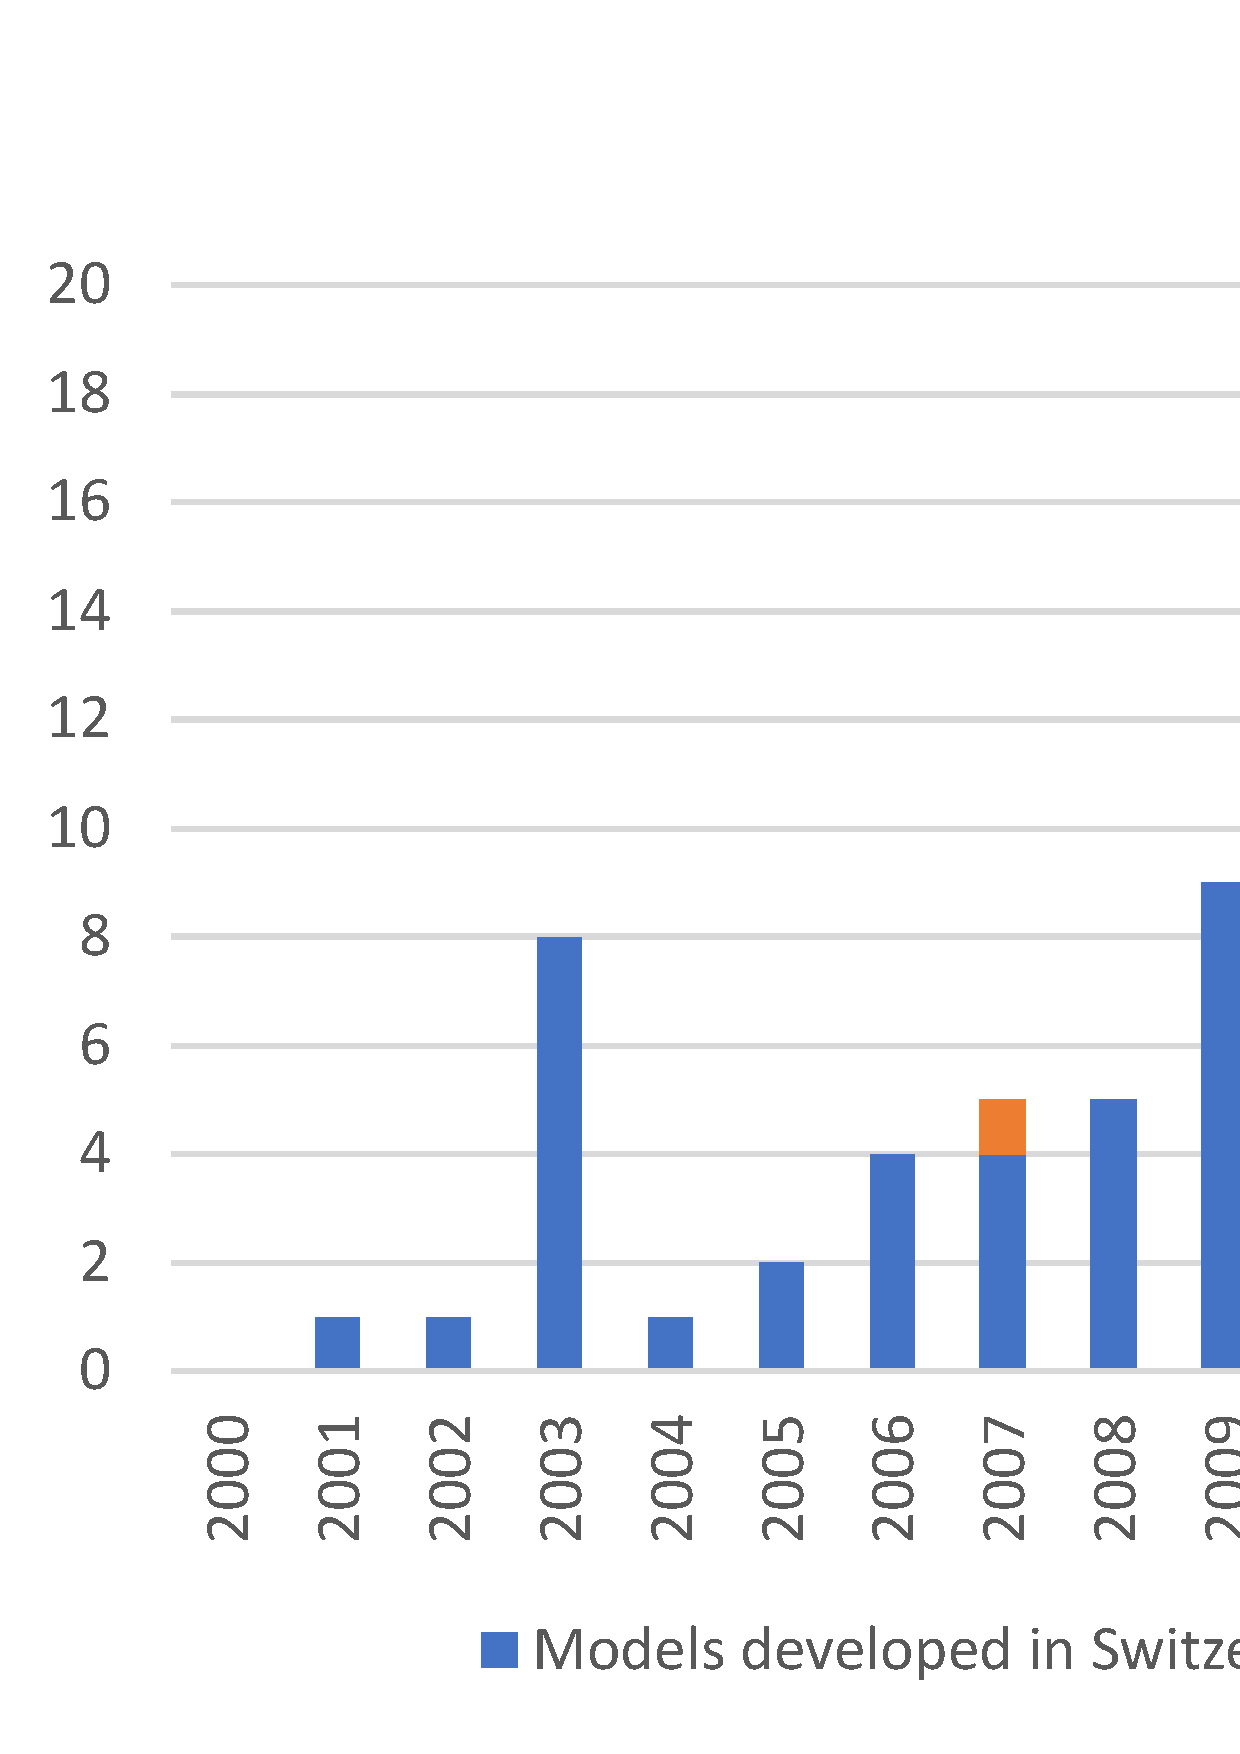
\includegraphics[width=0.55\columnwidth]{figures/histogram.png}
		\caption{{Number of articles reporting applications of hydrological models over the years with a distinction of the models developed in Switzerland and international models. The relatively higher peak in 2003 is mainly due to articles related to the MAP project (Mesoscale Alpine Programme).
		{\label{fig:bars}}
		}}
	\end{center}
\end{figure}
	
\setlength\extrarowheight{3pt}
\LTcapwidth=1.43\textwidth
\begin{longtable}{| P{4.8cm} | P{2.5cm}| P{4cm}| P{4cm}| X{1.2cm}| X{1.2cm}| X{1.2cm}| X{1.2cm}|}

\caption{List of reviewed modelling papers ordered by dates and author names. Adequacy: the adequacy of the model with the landscape or use case has been justified; Reuse: the model set up has been explicitly reused from previous work; Affiliation: the first author is affiliated with the institute where the model is being developed; Co-auth.: the model developer or its lead scientist is co-authoring the paper.}\\


\hline
\textbf{Reference}	&	\textbf{Model(s)}	&	\textbf{Field of application}	&	\textbf{Location}	&	\textbf{Adequacy}	&	\textbf{Reuse}	&	\textbf{Affiliation}	&	\textbf{Co-auth.}	\\ \hline

\citet{Middelkoop2001}	&	WaSIM	&	climate change, floods, droughts	&	Rhine	&	N	&	N	&	*	&	Y	\\
\citet{Jasper2002}	&	WaSIM	&	forecasting, floods	&	Ticino, Verzasca, Maggia	&	Y	&	N	&	Y	&	Y	\\
\citet{Ahrens2003}	&	WaSIM	&	forecasting	&	Ticino, Verzasca, Maggia	&	N	&	N	&	N	&	Y	\\
\citet{Ahrens2003a}	&	WaSIM	&	forecasting	&	Ticino, Verzasca, Maggia	&	N	&	Y	&	N	&	N	\\
\citet{Ahrens2003b}	&	WaSIM	&	forecasting	&	Ticino, Verzasca, Maggia	&	$+-$	&	N	&	N	&	N	\\
\citet{Gurtz2003}	&	PREVAH, WaSiM	&	others	&	Dischmabach, Rietholzbach	&	*	&	N	&	Y	&	Y	\\
\citet{Jasper2003}	&	WaSIM	&	forecasting	&	Ticino, Verzasca, Maggia	&	Y	&	N	&	Y	&	Y	\\
\citet{Verbunt2003}	&	WaSIM	&	cryosphere	&	Massa, Rhone, Dischmabach	&	$+-$	&	N	&	Y	&	Y	\\
\citet{Zappa2003}	&	PREVAH	&	others	&	Ticino	&	*	&	N	&	Y	&	Y	\\
\citet{Jasper2004}	&	WaSIM	&	climate change	&	Thur, Ticino	&	$+-$	&	N	&	Y	&	Y	\\
\citet{Kleinn2005}	&	WaSIM	&	climate change	&	Rhine	&	*	&	*	&	*	&	*	\\
\citet{Verbunt2005}	&	WaSIM	&	others	&	Swiss Alpine Rhine basin	&	$+-$	&	N	&	Y	&	Y	\\
\citet{Zierl2005}	&	RHESSys	&	climate change	&	Alptal, Saltina, Verzasca, Dischma	&	Y	&	N	&	N	&	N	\\
\citet{Calanca2006}	&	WaSIM	&	climate change	&	Thur, Ticino, Rhone	&	$+-$	&	N	&	Y	&	Y	\\
\citet{Horton2006}	&	GSM-SOCONT	&	climate change	&	11 catchments	&	N	&	N	&	Y	&	Y	\\
\citet{Jasper2006}	&	WaSIM	&	climate change	&	Thur	&	Y	&	N	&	Y	&	Y	\\
\citet{Verbunt2006}	&	PREVAH	&	forecasting, floods	&	Upper Rhine basin	&	Y	&	N	&	N	&	Y	\\
\citet{Abbaspour2007}	&	SWAT	&	others	&	Thur	&	N	&	N	&	N	&	Y	\\
\citet{Schaefli2007}	&	GSM-SOCONT	&	others	&	Mauvoisin	&	N	&	N	&	Y	&	Y	\\
\citet{Schaefli2007b}	&	GSM-SOCONT	&	climate change	&	Mauvoisin	&	N	&	N	&	Y	&	Y	\\
\citet{Verbunt2007}	&	PREVAH	&	forecasting, floods	&	Almost countrywide	&	$+-$	&	Y	&	N	&	N	\\
\citet{Zappa2007}	&	PREVAH	&	cryosphere, droughts	&	Thur, Rhone, Lütschine	&	$+-$	&	N	&	Y	&	Y	\\
\citet{Cullmann2008}	&	WaSIM	&	others	&	Rietholzbach	&	N	&	N	&	N	&	N	\\
\citet{Jaun2008}	&	PREVAH	&	forecasting, floods	&	Almost countrywide	&	N	&	N	&	N	&	N	\\
\citet{Zappa2008}	&	PREVAH	&	cryosphere	&	Whole Switzerland	&	*	&	N	&	Y	&	Y	\\
\citet{Zappa2008b}	&	PREVAH, HBV	&	forecasting, floods	&	Verzasca, Kleine Emme	&	*	&	*	&	Y	&	Y	\\
\citet{Bavay2009}	&	ALPINE3D	&	climate change, cryosphere	&	Dischma, Inn	&	Y	&	N	&	Y	&	Y	\\
\citet{Foglia2009}	&	TOPKAPI	&	others	&	Maggia valley	&	$+-$	&	N	&	N	&	N	\\
\citet{Foglia2009a}	&	TOPKAPI	&	others	&	Maggia valley	&	Y	&	N	&	N	&	N	\\
\citet{GarciaHernandez2009}	&	GSM-SOCONT, RS	&	forecasting, floods	&	Rhone	&	N	&	N	&	Y	&	Y	\\
\citet{Jaun2009}	&	PREVAH	&	forecasting	&	Upper Rhine basin	&	N	&	N	&	Y	&	N	\\
\citet{Schaefli2009}	&	GSM-SOCONT	&	others	&	Rhone	&	N	&	N	&	Y	&	Y	\\
\citet{Thielen2009}	&	LISFLOOD	&	forecasting, floods	&	European scale	&	*	&	*	&	*	&	*	\\
\citet{Viviroli2009a}	&	PREVAH	&	floods	&	Countrywide	&	Y	&	N	&	Y	&	Y	\\
\citet{Viviroli2009c}	&	PREVAH	&	floods	&	Upper Rhine basin	&	Y	&	N	&	Y	&	Y	\\
\citet{Hingray2010}	&	GSM-SOCONT	&	floods	&	Rhone	&	N	&	N	&	Y	&	Y	\\
\citet{Jordan2010}	&	GSM-SOCONT, RS	&	forecasting, floods	&	Rhone	&	N	&	N	&	Y	&	Y	\\
\citet{Koplin2010}	&	PREVAH	&	climate change, floods	&	Countrywide	&	Y	&	N	&	Y	&	Y	\\
\citet{Rossler2010}	&	WaSIM	&	others	&	Lonza (Lötschental valley)	&	*	&	N	&	N	&	N	\\
\citet{Addor2011}	&	PREVAH	&	forecasting, floods	&	Sihl catchment	&	N	&	Y	&	Y	&	Y	\\
\citet{Cullmann2011}	&	WaSIM	&	others	&	Thur	&	N	&	Y	&	N	&	N	\\
\citet{Finger2011}	&	TOPKAPI	&	cryosphere	&	Rhonegletscher	&	N	&	N	&	Y	&	Y	\\
\citet{Fundel2011}	&	PREVAH	&	forecasting	&	Thur, Alp, Verzasca	&	Y	&	N	&	Y	&	Y	\\
\citet{Hindshaw2011}	&	ALPINE3D	&	cryosphere, others	&	Damma glacier	&	$+-$	&	Y	&	N	&	N	\\
\citet{Junghans2011}	&	HBV, GERM	&	climate change, cryosphere	&	Upper Rhine basin	&	$+-$	&	N	&	N	&	Y	\\
\citet{Kobierska2011}	&	PREVAH, ALPINE3D	&	climate change, cryosphere	&	Damma glacier	&	N	&	N	&	Y	&	*	\\
\citet{Konz2011}	&	TOPKAPI	&	others	&	Chiene catchment	&	$+-$	&	N	&	Y	&	Y	\\
\citet{Schaefli2011}	&	GSM-SOCONT	&	cryosphere	&	Rhonegletscher	&	$+-$	&	N	&	Y	&	Y	\\
\citet{Tobin2011}	&	GSM-SOCONT	&	forecasting	&	Visp, Dranse	&	N	&	Y	&	Y	&	N	\\
\citet{Zappa2011a}	&	PREVAH	&	forecasting, floods	&	Verzasca	&	Y	&	N	&	Y	&	Y	\\
\citet{Farinotti2012}	&	GERM	&	climate change, cryosphere	&	9 catchments	&	*	&	N	&	N	&	Y	\\
\citet{Finger2012}	&	TOPKAPI	&	climate change, cryosphere	&	Vispa	&	N	&	N	&	Y	&	Y	\\
\citet{Fuhrer2012}	&	WaSIM	&	others	&	6 catchments	&	Y	&	N	&	Y	&	Y	\\
\citet{Koplin2012}	&	PREVAH	&	climate change	&	Whole Switzerland	&	N	&	N	&	Y	&	Y	\\
\citet{Rossler2012}	&	WaSIM	&	climate change, droughts	&	Lonza (Lötschental valley)	&	$+-$	&	Y	&	N	&	N	\\
\citet{Tobin2012}	&	GSM-SOCONT	&	forecasting	&	Rhone	&	N	&	N	&	Y	&	Y	\\
\citet{Bavay2013}	&	ALPINE3D	&	climate change, cryosphere	&	Grisons	&	Y	&	N	&	Y	&	Y	\\
\citet{Bieri2013}	&	GSM-SOCONT, RS	&	floods	&	Aare	&	N	&	N	&	Y	&	N	\\
\citet{Bosshard2013a}	&	PREVAH, HBV	&	climate change	&	Alpine Rhine	&	N	&	Y	&	N	&	Y	\\
\citet{Finger2013}	&	GERM	&	climate change, cryosphere	&	Glacier de la Plaine Morte	&	$+-$	&	N	&	N	&	Y	\\
\citet{Foglia2013}	&	TOPKAPI	&	others	&	Maggia valley	&	N	&	N	&	N	&	N	\\
\citet{Fundel2013}	&	PREVAH	&	forecasting, droughts	&	Thur	&	N	&	Y	&	Y	&	Y	\\
\citet{Kobierska2013}	&	PREVAH, ALPINE3D	&	climate change, cryosphere	&	Göscheralpsee	&	Y	&	Y	&	Y	&	Y	\\
\citet{Koplin2013}	&	PREVAH	&	climate change, cryosphere	&	Whole Switzerland	&	Y	&	Y	&	Y	&	Y	\\
\citet{Liechti2013}	&	PREVAH	&	forecasting, floods	&	Verzasca, Pincascia	&	N	&	N	&	Y	&	Y	\\
\citet{Rahman2013}	&	SWAT	&	others	&	Rhone	&	*	&	N	&	N	&	?	\\
\citet{Uhlmann2013}	&	GSM-SOCONT, RS	&	climate change, cryosphere	&	Findelen basin	&	$+-$	&	N	&	N	&	Y	\\
\citet{Addor2014}	&	HBV-light, PREVAH, WaSiM	&	climate change	&	6 catchments	&	*	&	*	&	*	&	*	\\
\citet{Alaoui2014}	&	WaSIM	&	climate change	&	Ursern Valley	&	$+-$	&	N	&	N	&	Y	\\
\citet{Bosshard2014}	&	PREVAH	&	climate change	&	Rhine	&	*	&	*	&	*	&	*	\\
\citet{Fatichi2014}	&	TOPKAPI	&	climate change	&	Rhone	&	Y	&	N	&	Y	&	Y	\\
\citet{Koplin2014}	&	PREVAH	&	climate change, floods	&	Whole Switzerland	&	N	&	N	&	Y	&	Y	\\
\citet{Koplin2014a}	&	PREVAH	&	climate change, cryosphere	&	Whole Switzerland	&	N	&	Y	&	Y	&	N	\\
\citet{Paschalis2014}	&	TOPKAPI	&	floods	&	Kleine Emme	&	Y	&	N	&	Y	&	Y	\\
\citet{Rahman2014}	&	SWAT	&	climate change	&	Rhone	&	$+-$	&	N	&	N	&	N	\\
\citet{Rossler2014}	&	WaSIM	&	floods	&	Lonza (Lötschental valley)	&	Y	&	Y	&	N	&	N	\\
\citet{Staudinger2014}	&	HBV-light	&	forecasting, droughts	&	21 catchments	&	N	&	N	&	Y	&	Y	\\
\citet{Staudinger2014a}	&	HBV-light	&	droughts, cryosphere	&	7 catchements	&	N	&	N	&	Y	&	Y	\\
\citet{Comola2015}	&	ALPINE3D	&	others	&	Dischma	&	N	&	N	&	Y	&	Y	\\
\citet{Comola2017}	&	ALPINE3D	&	cryosphere	&	Dischma	&	Y	&	N	&	Y	&	Y	\\
\citet{Fatichi2015}	&	TOPKAPI	&	climate change	&	Rhone	&	Y	&	N	&	Y	&	Y	\\
\citet{Finger2015}	&	HBV-light	&	cryosphere	&	Rhone, Hinterrhein, Landquart	&	$+-$	&	N	&	Y	&	Y	\\
\citet{Jorg-Hess2015}	&	PREVAH	&	forecasting, droughts	&	Landquart, Thur	&	N	&	Y	&	Y	&	Y	\\
\citet{Jorg-Hess2015a}	&	PREVAH	&	forecasting, cryosphere	&	Thur, Rhine, Hinter Rhine, Vorder Rhine, Vorarlberg, Landquart Plessur	&	N	&	Y	&	Y	&	Y	\\
\citet{Junker2015}	&	PREVAH	&	climate change	&	Kleine Emme	&	$+-$	&	Y	&	N	&	Y	\\
\citet{Milano2015}	&	PREVAH	&	climate change, droughts	&	9 catchments	&	N	&	N	&	N	&	N	\\
\citet{Milano2015a}	&	PREVAH	&	climate change	&	9 catchments in VD	&	Y	&	N	&	N	&	N	\\
\citet{Orth2015}	&	PREVAH, HBV	&	floods, droughts	&	Ergolz, Murg, Broye, Langeten, Cassarate, Sense, Emme, Dischma	&	$+-$	&	N	&	N	&	Y	\\
\citet{Pappas2015}	&	TOPKAPI	&	others	&	Kleine Emme	&	$+-$	&	N	&	Y	&	Y	\\
\citet{Rahman2015}	&	SWAT	&	climate change	&	Rhone	&	$+-$	&	Y	&	N	&	?	\\
\citet{RaymondPralong2015}	&	PREVAH	&	climate change	&	66 small catchments	&	$+-$	&	N	&	Y	&	Y	\\
\citet{Speich2015}	&	PREVAH	&	climate change, cryosphere	&	Countrywide	&	N	&	N	&	Y	&	Y	\\
\citet{Staudinger2015}	&	HBV-light	&	droughts	&	24 catchments	&	N	&	N	&	Y	&	Y	\\
\citet{Terrier2015}	&	GSM-SOCONT, RS	&	climate change	&	Aare	&	$+-$	&	Y	&	Y	&	Y	\\
\citet{Viviroli2015}	&	PREVAH	&	others	&	49 catchments	&	Y	&	N	&	Y	&	Y	\\
\citet{Andres2016}	&	PREVAH, RS	&	forecasting, floods	&	Canton Ticino	&	$+-$	&	Y	&	Y	&	Y	\\
\citet{Donnelly2016}	&	HYPE	&	others	&	European scale	&	*	&	*	&	*	&	*	\\
\citet{GironsLopez2016}	&	HBV-light	&	others	&	Thur	&	Y	&	N	&	Y	&	Y	\\
\citet{Griessinger2016}	&	HBV-light	&	forecasting, cryosphere	&	20 catchments	&	N	&	N	&	Y	&	Y	\\
\citet{Melsen2016}	&	VIC	&	others	&	Thur	&	$+-$	&	N	&	N	&	N	\\
\citet{Schaefli2016}	&	SEHR-ECHO	&	cryosphere	&	Dischma	&	N	&	N	&	Y	&	Y	\\
\citet{Sikorska2016}	&	HBV-light	&	forecasting, floods	&	Plessur	&	N	&	N	&	Y	&	Y	\\
\citet{Brauchli2017}	&	ALPINE3D	&	cryosphere	&	Dischma	&	Y	&	N	&	Y	&	Y	\\
\citet{Etter2017}	&	HBV-light	&	climate change, cryosphere	&	Gigerwaldsee	&	N	&	N	&	Y	&	N	\\
\citet{Felder2017}	&	PREVAH	&	floods	&	Aare	&	Y	&	N	&	Y	&	N	\\
\citet{Marty2017}	&	ALPINE3D	&	climate change, cryosphere	&	Aare, Grisons	&	N	&	N	&	Y	&	Y	\\
\citet{Sikorska2017}	&	HBV-light	&	floods	&	9 catchments	&	N	&	N	&	Y	&	Y	\\
\citet{Staudinger2017}	&	HBV-light	&	others	&	21 catchments	&	N	&	N	&	Y	&	Y	\\
\citet{VanOsnabrugge2017}	&	wflow\_hbv	&	forecasting	&	Rhine	&	*	&	*	&	*	&	*	\\
\citet{Wever2017}	&	ALPINE3D	&	cryosphere, floods	&	Dischma	&	Y	&	N	&	Y	&	Y	\\
\citet{Zeimetz2017}	&	GSM-SOCONT	&	floods	&	Mattmark	&	N	&	N	&	Y	&	Y	\\
\citet{Anghileri2018}	&	TOPKAPI	&	climate change, cryosphere	&	Visp	&	Y	&	N	&	Y	&	N	\\
\citet{Bogner2018}	&	PREVAH	&	forecasting, floods	&	Sihl catchment	&	N	&	Y	&	Y	&	Y	\\
\citet{Bogner2018b}	&	PREVAH	&	forecasting, droughts	&	Countrywide	&	N	&	N	&	Y	&	Y	\\
\citet{Brunner2018}	&	HBV-light	&	climate change, floods	&	8 catchments	&	$+-$	&	N	&	Y	&	Y	\\
\citet{Etter2018}	&	HBV-light	&	others	&	6 catchments	&	N	&	N	&	Y	&	Y	\\
\citet{Hakala2018a}	&	HBV-light	&	climate change	&	10 catchments	&	N	&	N	&	Y	&	Y	\\
\citet{Jenicek2018}	&	HBV-light	&	climate change, droughts, cryosphere	&	14 catchments	&	N	&	N	&	N	&	Y	\\
\citet{Meyer2018a}	&	HBV-light	&	climate change, cryosphere	&	Hinterrhein, Schwarze Lütschine	&	$+-$	&	N	&	N	&	Y	\\
\citet{Rossler2018}	&	WaSIM	&	floods	&	Rhine	&	N	&	N	&	N	&	N	\\
\citet{Shakoor2018}	&	ALPINE3D	&	cryosphere	&	Damma, Arolla	&	Y	&	N	&	Y	&	Y	\\
\citet{Sikorska2018}	&	HBV-light	&	others	&	13 catchments	&	N	&	N	&	Y	&	Y	\\
\citet{Stucki2018}	&	PREVAH, RS	&	floods	&	Lago Maggiore	&	N	&	Y	&	N	&	N	\\
\citet{Zarrineh2018}	&	SWAT	&	others	&	Broye	&	$+-$	&	N	&	N	&	N	\\
\citet{Zeimetz2018}	&	GSM-SOCONT	&	floods	&	Mattmark	&	N	&	Y	&	Y	&	Y	\\
\citet{Zeimetz2018a}	&	GSM-SOCONT, RS	&	floods, cryosphere	&	Mattmark Dam	&	N	&	N	&	Y	&	Y	\\
\citet{Zischg2018}	&	PREVAH	&	floods	&	Aare	&	N	&	Y	&	Y	&	N	\\
\citet{Ancey2019}	&	GERM	&	cryosphere	&	Giétro	&	N	&	N	&	N	&	Y	\\
\citet{Andrianaki2019}	&	SWAT	&	cryosphere	&	Damma glacier watershed	&	*	&	N	&	N	&	N	\\
\citet{Anghileri2019}	&	PREVAH	&	forecasting	&	Verzasca	&	Y	&	Y	&	N	&	Y	\\
\citet{Antonetti2019}	&	PREVAH	&	forecasting, floods	&	Emme	&	N	&	N	&	Y	&	Y	\\
\citet{Brunner2019}	&	PREVAH	&	droughts	&	Countrywide	&	N	&	N	&	Y	&	Y	\\
\citet{Brunner2019a}	&	PREVAH	&	climate change, droughts	&	Countrywide	&	Y	&	N	&	Y	&	Y	\\
\citet{Brunner2019b}	&	HBV-light	&	floods	&	9 catchments	&	N	&	N	&	N	&	N	\\
\citet{Brunner2019c}	&	PREVAH	&	climate change, floods, droughts	&	19 regions	&	N	&	Y	&	Y	&	Y	\\
\citet{Brunner2019d}	&	PREVAH	&	climate change, floods	&	Countrywide	&	Y	&	N	&	Y	&	Y	\\
\citet{Brunner2019e}	&	PREVAH	&	droughts	&	Countrywide	&	Y	&	Y	&	Y	&	Y	\\
\citet{Keller2019}	&	GR6J	&	climate change, floods	&	Emme	&	N	&	N	&	N	&	N	\\
\citet{Keller2019a}	&	WaSIM	&	climate change, floods	&	Thur	&	N	&	N	&	N	&	N	\\
\citet{Mastrotheodoros2019}	&	VIC	&	floods, droughts	&	Thur	&	$+-$	&	N	&	N	&	N	\\
\citet{Melsen2019}	&	VIC	&	others, floods, droughts	&	Thur	&	N	&	Y	&	N	&	N	\\
\citet{Monhart2019}	&	PREVAH	&	forecasting	&	Verzasca, Thur, Klöntal	&	N	&	N	&	Y	&	Y	\\
\citet{Muller-Thomy2019}	&	HBV-light	&	floods	&	9 catchments	&	N	&	N	&	N	&	N	\\
\citet{Rossler2019}	&	WaSIM	&	climate change	&	Thur	&	N	&	N	&	N	&	N	\\
\citet{VanOsnabrugge2019}	&	wflow\_hbv	&	forecasting	&	Rhine	&	*	&	*	&	*	&	*	\\
\citet{Wanders2019}	&	mHM	&	forecasting	&	European scale	&	*	&	*	&	*	&	*	\\
\citet{Battista2020}	&	TOPKAPI	&	others	&	Kleine Emme	&	Y	&	N	&	Y	&	N	\\
\citet{Battista2020a}	&	TOPKAPI	&	others	&	Kleine Emme	&	Y	&	N	&	Y	&	N	\\
\citet{DalMolin2020}	&	SUPERFLEX	&	others	&	Thur	&	*	&	N	&	Y	&	Y	\\
\citet{Etter2020}	&	HBV-light	&	others	&	Murg, Guerbe, Mentue, Verzasca	&	N	&	N	&	Y	&	Y	\\
\citet{Giordani2020}	&	PREVAH	&	forecasting, floods	&	Verzasca	&	N	&	Y	&	N	&	Y	\\
\citet{Hakala2020}	&	HBV-light	&	climate change, floods, droughts	&	Montsalvens, Vernex	&	N	&	N	&	Y	&	Y	\\
\citet{Rottler2020}	&	mHM	&	climate change, floods	&	Rhine	&	*	&	*	&	*	&	*	\\
\citet{Sikorska-Senoner2020}	&	HBV	&	floods	&	Dünnern at Olten	&	$+-$	&	N	&	Y	&	Y	\\
\citet{Westerberg2020}	&	HBV-light	&	others	&	Kander, Broye, Wigger	&	N	&	N	&	N	&	Y	\\
\citet{Zarrineh2020}	&	SWAT	&	climate change	&	Broye	&	N	&	Y	&	N	&	N	\\
\citet{Thornton2021}	&	WaSIM	&	cryosphere	&	Vallon de Nant	&	Y	&	N	&	N	&	N	\\


\hline
\multicolumn{8}{l}{* not relevant or not analysed}\\

\end{longtable}
\label{table:articles}

\end{landscape}

\section*{Acknowledgement}

We would like to thank Jean-Pierre Jordan, Anton Schleiss, Manfred Stähli and Ludwig Braun for their references for this part. 


\bibliographystyle{ametsoc2014}
%\bibliographystyle{plain}
\bibliography{Refs_suppmat}
\end{document}
